\chapter{Thuật toán Q-Learning và Deep Q-Learning}
\label{ch:04}
\section{Q-Learning}
\subsection{Giới thiệu}
Những thuật toán học tăng cường thông thường gồm có quy hoạch động (Dynamic
Programming), Monte-Carlo và phương pháp TD (Temporal-Difference). Tuy nhiên các phương
pháp quy hoạch động và Monte-Carlo không hiệu quả do đòi hỏi bộ nhớ quá lớn, hoặc mô hình
phải xác định hay khó hội tụ nên ít khi cho ra kết quả tối ưu. Phương pháp TD là sự kết hợp của
hai phương pháp quy hoạch động, Monte-Carlo và nó còn cho phép giải quyết được nhiều bài toán thực tế bởi vì phương
pháp này không đòi hỏi môi trường xác định và có khả năng hội tụ cao. Một biến thể của
phương pháp TD được gọi là Q-learning. Nó là một phương pháp học kiểu TD theo hướng off-policy,
rất hiệu quả trong việc giải quyết các bài toán tìm đường. Quá trình học tăng cường có thể được thực
hiện theo hai cách: off-policy và on-policy. On-policy sử dụng một chiến lược chọn hành động để thực
hiện các bước hành động để tối ưu hóa chính chiến lược chọn hành động đó. Phương pháp off-policy
sử dụng một chiến lược chọn hành động để thực hiện các hành động nhưng với mục đích là để tối ưu
hóa một chiến lược chọn hành động khác.
\subsection{Thuật toán Q-Learning}
Cho một chiến lược (policy) $\pi$, ta viết lại công thức (trình bày ở chương 3) về Q-value (hay là giá trị hành động)
như sau:
\begin{equation} 
    \label{eq:Qvalue}
    Q^{\pi}(s,a) = R(s,a) + \gamma \sum_{s'\in \S} P_{ss^{'}}^{a}V^{\pi}(s').
\end{equation}
Trong công thức \ref{eq:Qvalue}, $Q^{\pi}(s,a)$ là Q-value khi thực hiện hành động a tại trạng thái s theo chiến lược $\pi$; $R(s,a)$ là phần thưởng nhận được; $s^{'}$ là trạng thái kế tiếp. $\gamma$ là hệ số giảm (discount rate), đảm bảo "gần" đích Q-value càng lớn.\\
Nói các khác, Q-value là hàm giá trị hành động mong đợi cho việc thực hiện hành động $a$ ở trạng thái $s$ và tuân theo chính sách $\pi$ sau đó. 
 Mục đích của Q-learning là ước lượng Q-values cho một chiến lược tối ưu. Để tiện lợi, ta định nghĩa như sau 
 $Q^{*}(s,a) \equiv Q^{\pi^{*}}(s,a), \forall s, a$. Thật đơn giản để chỉ ra rằng
  $V^{*}(s) = max_{a} Q^{*}(s,a)$ và nếu $a^{*}$ là một hành động mà tại đó
  mức tối đa đạt được, sau đó một chiến lược tối ưu có thể được hình thành như $\pi^{*}(s) \equiv a^{*}$.
  Ở đây, lợi ích của những giá trị Q-value là nếu một tác tử (agent) có thể học chúng, nó có thể 
  dễ dàng quyết định đâu là tối ưu để hành động. Mặc dù có thể có nhiều hơn một chiến lược tối ưu hay 
  $a^{*}$, những giá trị $Q^{*}$ là duy nhất.\\
  \indent Trong Q-learning,  kinh nghiệm của tác tử (agent) bao gồm một chuỗi tuần tự các quá trình riêng biệt (gọi là Episodes).\\
  Trong episode thứ n, tác tử sẽ:
\begin{itemize}
    \item quan sát trạng thái hiện tại của nó $s_n$,
    \item lựa chọn và thực hiện một hành động $a_n$,
    \item quan sát trạng thái tiếp theo $s_{n+1}$,
    \item nhận được ngay phần thưởng $r_n$, và
    \item điều chỉnh các giá trị $Q_{n-1}$ của nó bằng cách sử dụng hệ số học $\alpha_{n}$, theo:
\end{itemize}
\begin{equation} 
Q_{n}(s,a) =  \begin{cases}
    (1-\alpha_n)Q_{n-1}(s,a) + \alpha_{n}[r_n + \gamma V_{n-1}(s_{n+1})] &\text{nếu } s = s_n \text{ và } a = a_n,\\
    Q_{n-1}(s, a) &\text{trường hợp khác}
\end{cases}   
\end{equation}
Trong đó :
\begin{equation} 
    \label{eq:Vn}
    V_{n-1}(s) \equiv max_{b} {Q_{n-1}(s,b)}
\end{equation}
là tốt nhất mà tác tử có thể làm được từ trạng thái s. Dĩ nhiên, ở những giai đoạn đầu việc học thì Q-value có thể không phản ánh 
đúng chiến lược mà chúng đã được biết (việc tối đa hóa các hành động ở phương trình \ref{eq:Vn}). 
Hiển nhiên là các giá trị Q-value ban đầu, $Q_{0}(s,a)$, cho tất cả các trạng thái và hành động đã được giả thiết. Ngoài ra ta có thêm 
giải thiết một bảng tra cứu (look-up table) biểu diễn cho $Q_n(s,a)$. 
Theo ~\cite{Watkins1989} cho thấy Q-learning có thể không hội tụ chính xác cho các biểu diễn khác.\\
\indent Phân tích thuật toán Q-learning, ta có các bước như sau:
\begin{itemize}
    \item 1. Khởi tạo bảng Q với các số 0 và giá trị Q thành các hằng số tùy ý.
    \item 2. Khám phá các hành động: đối với mỗi thay đổi về trạng thái, chọn bất 
    kỳ một hành động (a) nào trong số tất cả các hành động có thể có cho trạng thái 
    hiện tại (S).
    \item 3. Đi đến trạng thái tiếp theo (S') là kết quả của hành động (a).
    \item 4. Đối với tất cả các hành động có thể từ trạng thái (S,), hãy chọn một hành 
    động có giá trị Q cao nhất.
    \item 5. Cập nhật giá trị bảng Q bằng phương trình.
    \item 6. Đặt trạng thái tiếp theo làm trạng thái hiện tại.
    \item 7. Nếu trạng thái cuối đạt được, sau đó kết thúc và lặp lại quá trình.
\end{itemize}
\subsection{Sự hội tụ của thuật toán}
Điều kiện quan trọng nhất trong định lý hội tụ được đưa ra dưới đây là chuỗi các quá trình (Episodes) hình thành nền tảng học tập phải 
bao gồm vô hạn quá trình cho mỗi trạng thái và hành động bắt đầu. Đây có thể được coi là một điều kiện mạnh về cách lựa chọn các 
trạng thái và hành động, tuy nhiên, trong các điều kiện ngẫu nhiên của định lý, không có phương pháp nào có thể được đảm bảo 
để tìm ra một chiến lược tối ưu trong các điều kiện yếu hơn. Tuy nhiên, xin lưu ý rằng các quá trình không cần phải tạo thành một 
chuỗi liên tục, đó là $y$ của một quá trình không cần phải là $x$ của quá trình tiếp theo.\\
\indent Định lý dưới đây định nghĩa một tập các điều kiện theo đó $Q_n(s,a) \to Q^{*}(s,a)$ khi $n \to \infty$. 
Định nghĩa $n^{i}(s, a)$ là chỉ số của lần thứ i mà hành động a được thử ở trạng thái s.
Định lý hội tụ thuật toán Q-learning:
\begin{theorem}
    \label{th:Conver}
    Cho một miền phần thưởng bị chặn $r_n \leq R$, tỉ lệ học $0 \leq \alpha_n < 1$, và
    \begin{equation}
        \sum_{i=1}^{\infty}\alpha_{n^{i}(s,a)} = \infty, \sum_{i=1}^{\infty}[\alpha_{n^{i}(s,a)}]^2 < \infty, \forall s, a,
    \end{equation} 
    thì $Q_n(s,a) \to Q^{*}(s,a)$ khi $n \to \infty, \forall x, a,$ với xác suất bằng 1.
\end{theorem}
Chứng minh tính đúng đắn của định lý \ref{th:Conver} xem chi tiết trong~\cite{Watkins1992}.
\section{Deep Q-Learning}
Mục đích của bài toán là chọn ra hành động (action) thích hợp cho một trạng thái nào đó (state) 
nào đó. Hay nói cách khác, với state là đầu vào và cần đầu ra là một hành động. 
Công việc đó sẽ được thực hiện qua một mang nơ-ron (Neural Network-NN). Những gì ta cần làm 
chỉ là bỏ đi  bảng tra cứu lookup table $Q(s,a)$ và thay thế bằng một mạng nơ-ron đơn giản. 
Điều đó được mô tả trong Hình \ref{fig:qlearning}.
\begin{figure}[ht]
    \centering
    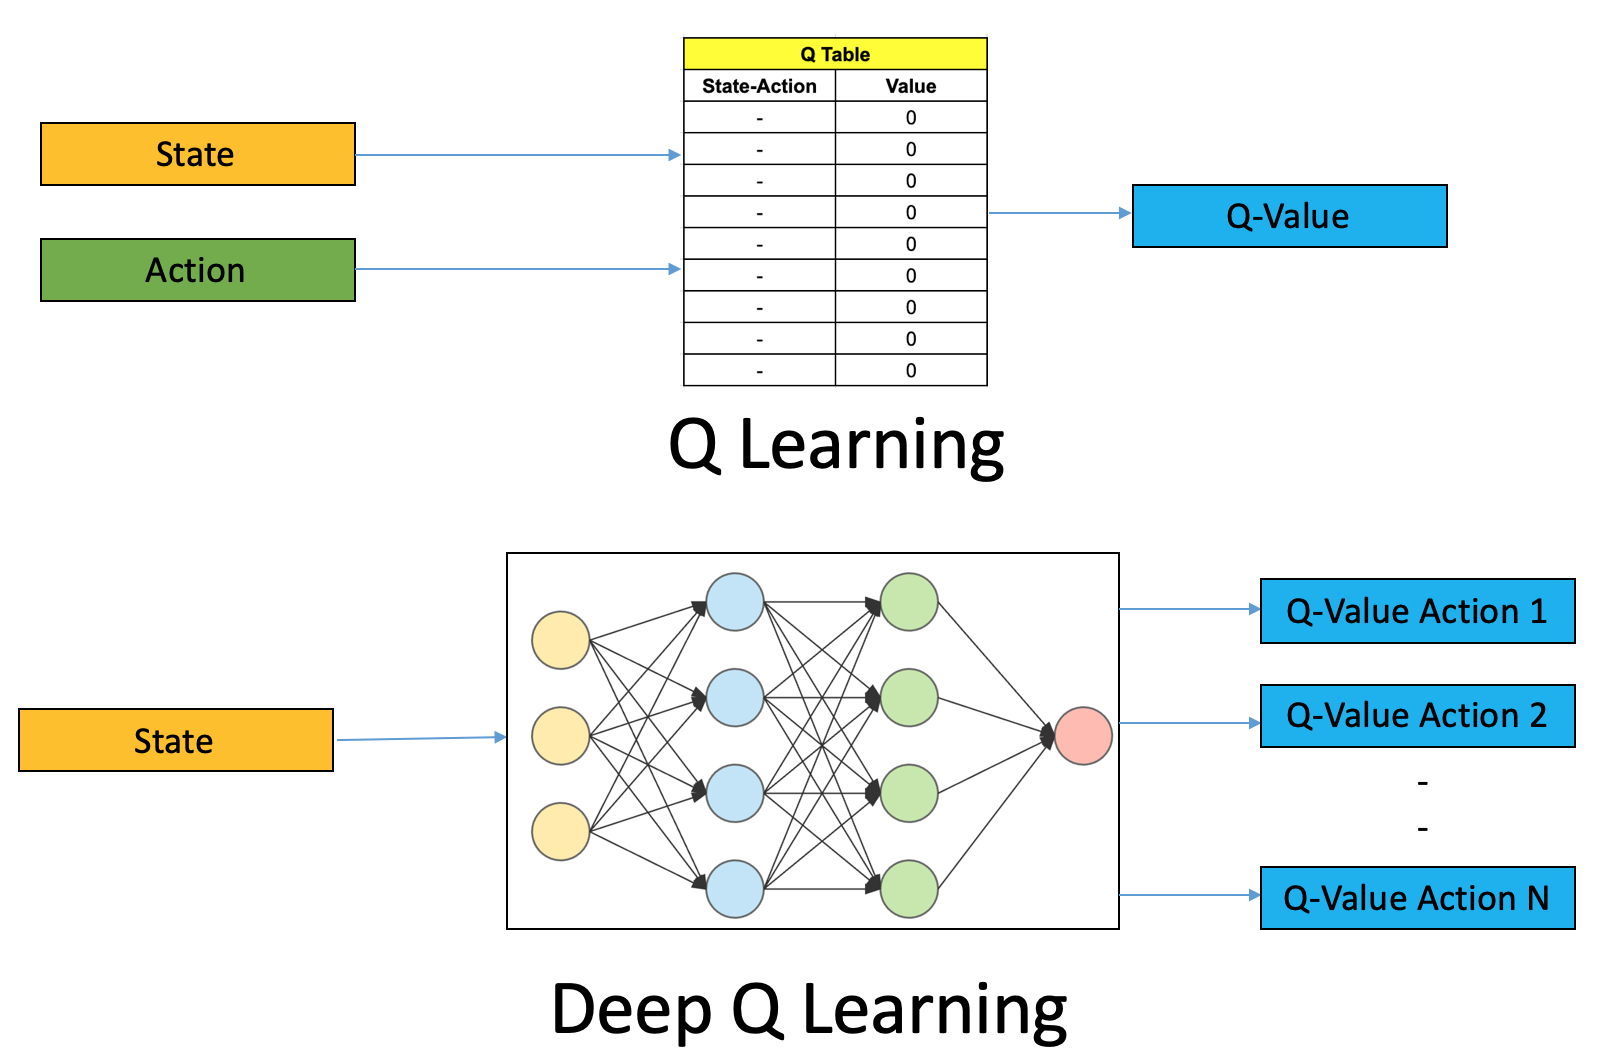
\includegraphics[width=\textwidth]{qvsdeepQlearning.png}
    \caption{So sánh về cấu trúc giữa Q-learning và Deep Q-learning.}
    \label{fig:qlearning}
\end{figure}
\subsubsection{Hàm mất mát}
Mục đích của ta là bắt mạng học được cách ước lượng Q-Value cho các hành động một cách chính xác nên đương nhiên 
hàm mất mát phải tính được sai số giữa Q-value thực tế và dự đoán. Hàm mất mát định nghĩa dưới dạng đầy đủ 
như sau:
\begin{equation}
    \label{eq:lossf}
    Loss = (r + \gamma max_{a'}Q(s', a'; \theta') - Q(s, a; \theta))^2
\end{equation}
\subsubsection{Kinh nghiệm chơi lại (Experience replay)} 
Ở phần trên ta đã định nghĩa một mạng nơ-ron lấy input là state hiện tại và output các Q-value. 
Thế nhưng nếu mạng nơ-ron  cứ liên tục bị đẩy vào từng state một sẽ rất dễ bị overfitting 
vì các states liên tục thường giống nhau hoặc có tính tuyến tính (ví dụ: liên tục 
đi thẳng/sang trái/phải). Kỹ thuật Experience Replay được sử dụng để loại bỏ vấn đề này.
 Thay vì mỗi state mạng update một lần, ta lưu lại các states vào bộ nhớ (memory).
 Sau đó thực hiện sampling thành các batch nhỏ đưa vào mạng nơ-ron học. Việc này giúp đa 
 dạng hóa input và tránh mạng nơ-ron bị overfitting.
 \subsubsection{Mô hình}
 Mô hình đầy đủ của Deep Q-Learning được mô tả trong Hình \ref{fig:deepqlearning}
 \begin{figure}[ht]
    \centering
    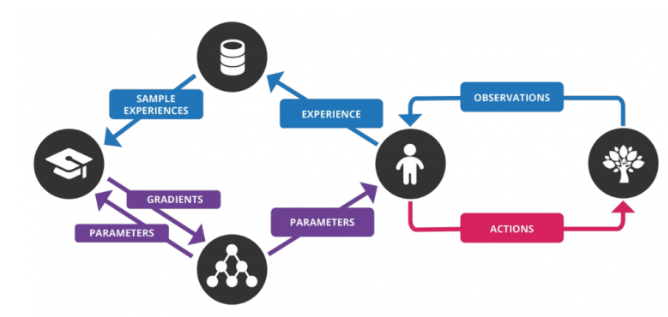
\includegraphics[width=\textwidth]{model.png}
    \caption{Mô hình Deep Q-Learning.}
    \label{fig:deepqlearning}
\end{figure}
\subsubsection{\underline{Tóm lại}}
Deep Q-Learning thực hiện các bước sau:
\begin{itemize}
    \item 1. Enviroment đưa vào mạng một state s; đầu ra là các Q-value của các actions tương ứng.
    \item 2. Agent chọn action bằng một Policy và thực hiện action a đó.
    \item 3. Environment trả lại state s' cùng với reward r tương ứng và lưu lại experience s, a, r, s'.
    \item 4. Thực hiện sample các experience thành một vài batches và tiến hành luyện mạng.
    \item 5. Lặp lại đến khi kết thúc M episodes.
\end{itemize}